%%%%%%%%%%%%%%%%%%%%%%%%%%%%%%%%%%%%%%%%%%%%%%%%%%%%%%%%%%%%%%%%%%%%%%%%%%%%%%%%

\talksection{What \& why: LLVM}

\begin{frame}{What is LLVM?}

\begin{itemize}
    \item Collection of modular compiler and toolchain technologies
    \item Started as a research project
    \item Apple took it on in 2005
    \item Grown to include many sub-projects:
    \begin{itemize}
      \item LLVM Core - Optimizers, code generators
      \item Clang     - C/C++/Objective-C front-end
      \item LLDB      - Debugger
      \item libc++    - Conformant \& performant C++ STL
      \item lld       - System linker
    \end{itemize}
\end{itemize}

\end{frame}

%%%%%%%%%%%%%%%%%%%%%%%%%%%%%%%%%%%%%%%%%%%%%%%%%%%%%%%%%%%%%%%%%%%%%%%%%%%%%%%%

\begin{frame}{Why LLVM?}

\begin{itemize}
    \item Open source
    \item Nice, permissive license
    \item Modular
    \item Active community
\end{itemize}

\end{frame}

%%%%%%%%%%%%%%%%%%%%%%%%%%%%%%%%%%%%%%%%%%%%%%%%%%%%%%%%%%%%%%%%%%%%%%%%%%%%%%%%

\talksection{Our backend: LEG}

\begin{frame}{Example target: LEG}

\begin{itemize}
    \item Simple, RISC-like architecture
    \begin{itemize}
        \item Very small subset of ARM
    \end{itemize}
    \item 12 integer registers (32-bit)
    \begin{itemize}
        \item r0, r1, ..., r9, sp (stack pointer), lr (return address)
    \end{itemize}
    \item Instructions:
    \begin{itemize}
        \item 32-bit arithmetic (add, subtract, multiply, mad)
        \item 32-bit register move, 16-bit constant moves
        \item 32-bit load/store
        \item integer comparison, branch, branch and link
    \end{itemize}
\end{itemize}

\end{frame}

%%%%%%%%%%%%%%%%%%%%%%%%%%%%%%%%%%%%%%%%%%%%%%%%%%%%%%%%%%%%%%%%%%%%%%%%%%%%%%%%

\begin{frame}[fragile]{LEG assembly examples}

\begin{itemize}
    \item Function that adds two integers
    \begin{itemize}
        \item The arguments are passed in registers: \texttt{a} in \texttt{r0}, \texttt{b} in \texttt{r1}
        \item The return value is stored in \texttt{r0}
    \end{itemize}
    \item Returns to the caller using \texttt{b}
    \begin{itemize}
        \item \texttt{lr} contains the function's return address
    \end{itemize}
\end{itemize}

\begin{minipage}[t]{0.50\linewidth}
\begin{codebox}
int foo(int a, int b) {
    int result = a + b;   // r0 + r1
    return result;        // r0
}
\end{codebox}
\codecaption{ex1.c}
\end{minipage}
\begin{minipage}[t]{0.49\linewidth}
\begin{codebox}
.foo:
    add r0, r0, r1
    b lr

\end{codebox}
\codecaption{ex1.s}
\end{minipage}

\end{frame}

%%%%%%%%%%%%%%%%%%%%%%%%%%%%%%%%%%%%%%%%%%%%%%%%%%%%%%%%%%%%%%%%%%%%%%%%%%%%%%%%

\begin{frame}[fragile]{LEG assembly examples}

\begin{itemize}
    \item Function that loads a value, adds a constant and stores the result
    \begin{itemize}
        \item \texttt{ldr} loads a value from memory at the given address
        \item \texttt{mov} copies an immediate value to the register
        \item \texttt{str} stores a value to memory at the given address
    \end{itemize}
\end{itemize}

\begin{minipage}[t]{0.50\linewidth}
\begin{codebox}
void ex7(int *src, int *dst) {
    int x = src[0];
    int result = x + 42;
    dst[0] = result;
}

\end{codebox}
\codecaption{ex7.c}
\end{minipage}
\begin{minipage}[t]{0.49\linewidth}
\begin{codebox}
ex7:
    ldr r0, [r0]
    mov r2, #42
    add r0, r0, r2
    str r0, [r1]
    bx lr
\end{codebox}
\codecaption{ex7.s}
\end{minipage}

\end{frame}

%%%%%%%%%%%%%%%%%%%%%%%%%%%%%%%%%%%%%%%%%%%%%%%%%%%%%%%%%%%%%%%%%%%%%%%%%%%%%%%%

\begin{frame}[fragile]{LEG assembly examples}

\begin{itemize}
    \item Function that either adds or subtracts two integers
    \item The result depends on which argument is greater
    \begin{itemize}
        \item \texttt{cmp} compares the arguments
        \item \texttt{b} branches to the '\texttt{if\_else}' basic block, using:
        \begin{itemize}
            \item The '\texttt{le}' predicate
            \item The implicit condition flag register set by \texttt{cmp}
        \end{itemize}
        \item Fall-through to '\texttt{if\_then}' if the predicate doesn't match
    \end{itemize}
\end{itemize}

\begin{minipage}[t]{0.50\linewidth}
\begin{codebox}
int ex6(int a, int b) {
    if (a > b) {
        return a + b;
    } else {
        return a - b;
    }
}


\end{codebox}
\codecaption{ex6.c}
\end{minipage}
\begin{minipage}[t]{0.49\linewidth}
\begin{codebox}
.ex6:
    cmp r0, r1
    ble .if_else
.if_then:
    add r0, r0, r1
    bx lr
.if_else:
    sub r0, r0, r1
    bx lr
\end{codebox}
\codecaption{ex6.s}
\end{minipage}

\end{frame}

%%%%%%%%%%%%%%%%%%%%%%%%%%%%%%%%%%%%%%%%%%%%%%%%%%%%%%%%%%%%%%%%%%%%%%%%%%%%%%%%

\talksection{LLVM Backend: The big picture}

\begin{frame}{LLVM Backend: The big picture}

\begin{itemize}
    \item Pipeline structure
    \begin{itemize}
        \item Transforms your program many times using different stages
        \item Starts target-independent, then gets increasingly target-specific
    \end{itemize}
    \item Different representations are used
    \begin{itemize}
        \item Tells you roughly where you are in the pipeline
        \item Different instruction namespaces
    \end{itemize}
    \item Check it out (IR and MI representations only):
    \begin{itemize}
        \item \texttt{llc foo.ll -print-after-all 2>\&1 > foo.log}
    \end{itemize}
\end{itemize}

\pipelinemap{IR → SelectionDAG → MachineDAG → MachineInstr → MCInst}{15.5ex}

\end{frame}

%%%%%%%%%%%%%%%%%%%%%%%%%%%%%%%%%%%%%%%%%%%%%%%%%%%%%%%%%%%%%%%%%%%%%%%%%%%%%%%%

\begin{frame}[fragile]{A look at an IR module}

\begin{itemize}
    \item Linear representation
    \begin{itemize}
        \item Basic blocks are lists of instructions
        \item Control Flow Graph (CFG) of basic blocks
    \end{itemize}
    \item High-level, target-agnostic
    \begin{itemize}
        \item Exceptions: data layout, triple, intrinsics
    \end{itemize}
    \item Most instructions define values
    \begin{itemize}
        \item Typed (e.g. \texttt{i32}, \texttt{float}, \texttt{<4 x i32>})
        \item Defined once (SSA), no registers
    \end{itemize}
\end{itemize}

\begin{codebox}
target datalayout = "e-m:e-p:32:32-i1:8:32-i8:8:32-i16:16:32-i64:32-f64-..."
target triple = "leg"

define i32 @foo(i32 %a, i32 %b) {
    %c = add i32 %a, %b
    ret i32 %c
}
\end{codebox}
\codecaption{ex1b.ll}

\pipelinemap{\codeempha{IR} → SelectionDAG → MachineDAG → MachineInstr → MCInst}{0.0ex}

\end{frame}

%%%%%%%%%%%%%%%%%%%%%%%%%%%%%%%%%%%%%%%%%%%%%%%%%%%%%%%%%%%%%%%%%%%%%%%%%%%%%%%%

\begin{frame}{A look at a SelectionDAG graph}

\begin{minipage}[t]{0.50\linewidth}
    \begin{itemize}
        \item Graph representation
        \item Operations as nodes
        \begin{itemize}
            \item Mostly target-agnostic
            \begin{itemize}
                \item Semantics defined by LLVM
                \item ISD namespace for opcodes
            \end{itemize}
            \item Produce typed value(s)
        \end{itemize}
        \item Dependencies as edges
        \begin{itemize}
            \item Data
            \item \codeemphb{Order ("chain")}
            \item \codeempha{Scheduling ("glue")}
        \end{itemize}
    \end{itemize}
\end{minipage}
\begin{minipage}[t]{0.49\linewidth}
    \begin{figure}
        \vspace{-2.2ex}
        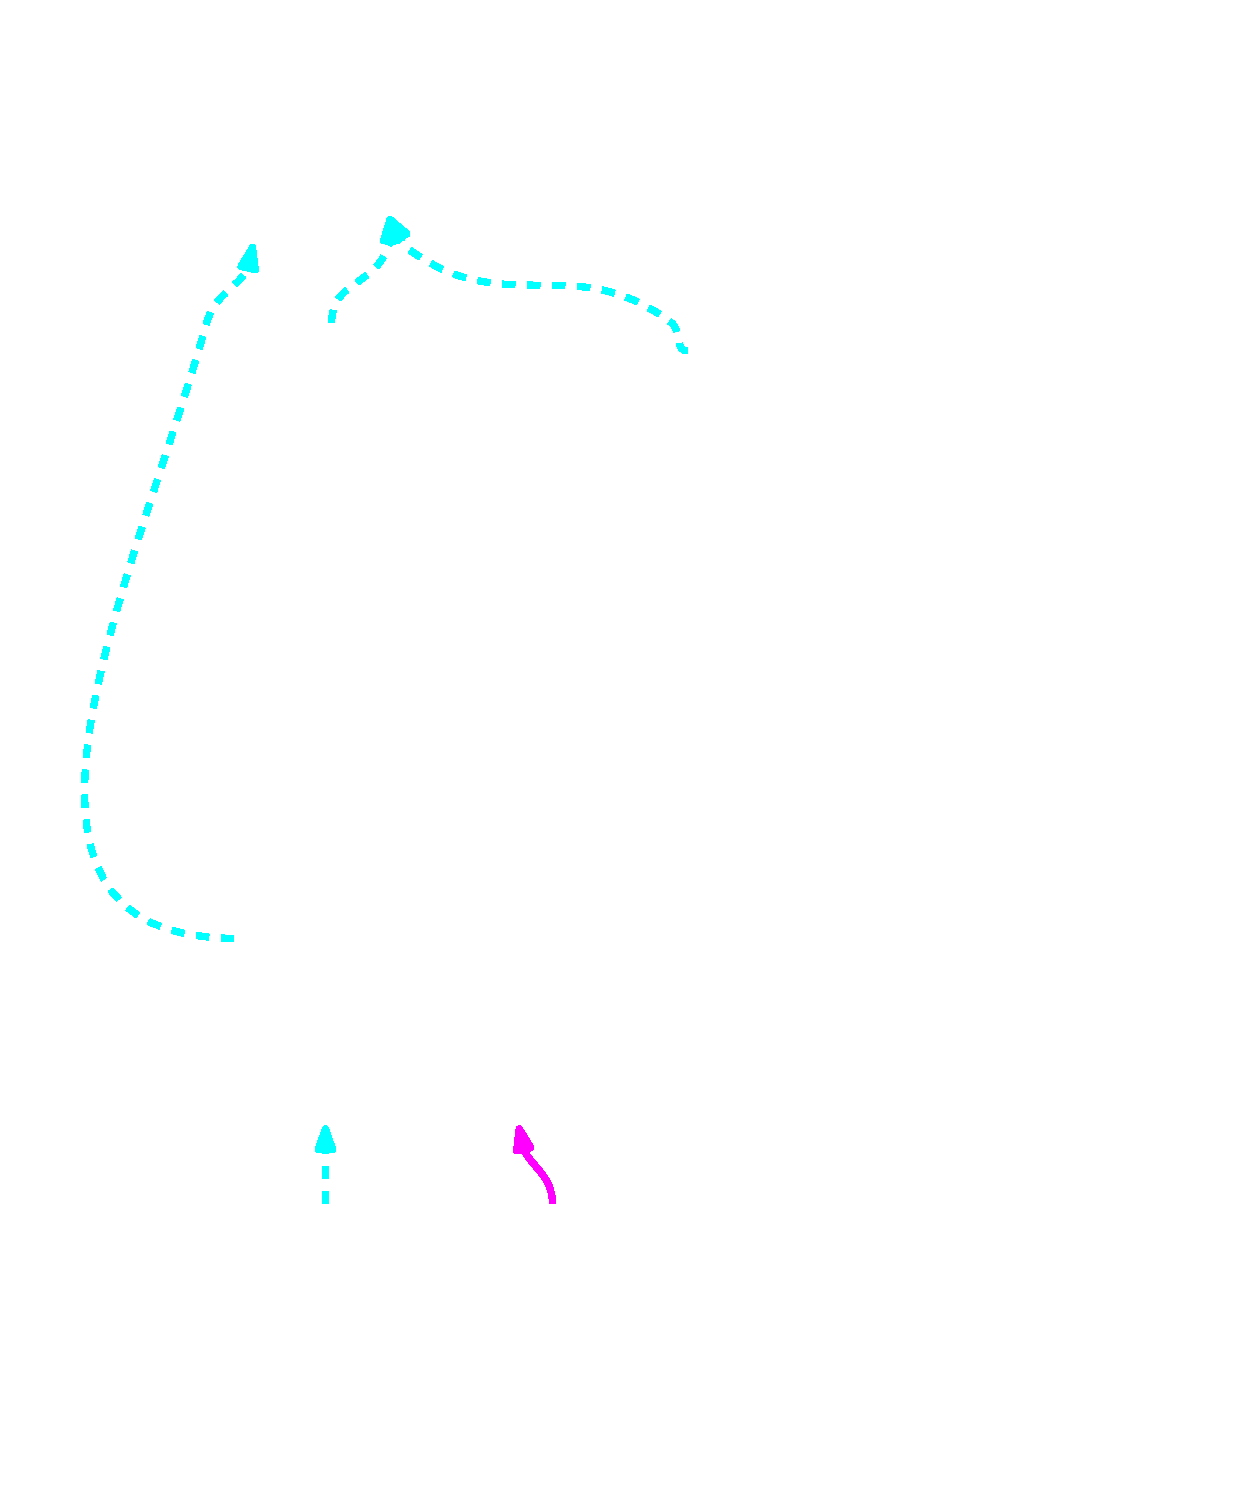
\includegraphics[width = 1.0\textwidth]{examples/ex1b/ex1b-pre-isel.pdf}
    \end{figure}
\end{minipage}

\pipelinemap{IR → \codeempha{SelectionDAG} → MachineDAG → MachineInstr → MCInst}{7.9ex}

\end{frame}

%%%%%%%%%%%%%%%%%%%%%%%%%%%%%%%%%%%%%%%%%%%%%%%%%%%%%%%%%%%%%%%%%%%%%%%%%%%%%%%%

\begin{frame}{A look at a MachineDAG graph}

\begin{minipage}[t]{0.50\linewidth}
    \begin{itemize}
        \item Very similar to SelectionDAG
        \item Target instructions as nodes
        \begin{itemize}
            \item Result of instruction selection
            \item LEG namespace
        \end{itemize}
        \item Similar dependencies
        \item Similar types
    \end{itemize}
\end{minipage}
\begin{minipage}[t]{0.49\linewidth}
    \begin{figure}
        \vspace{-2.2ex}
        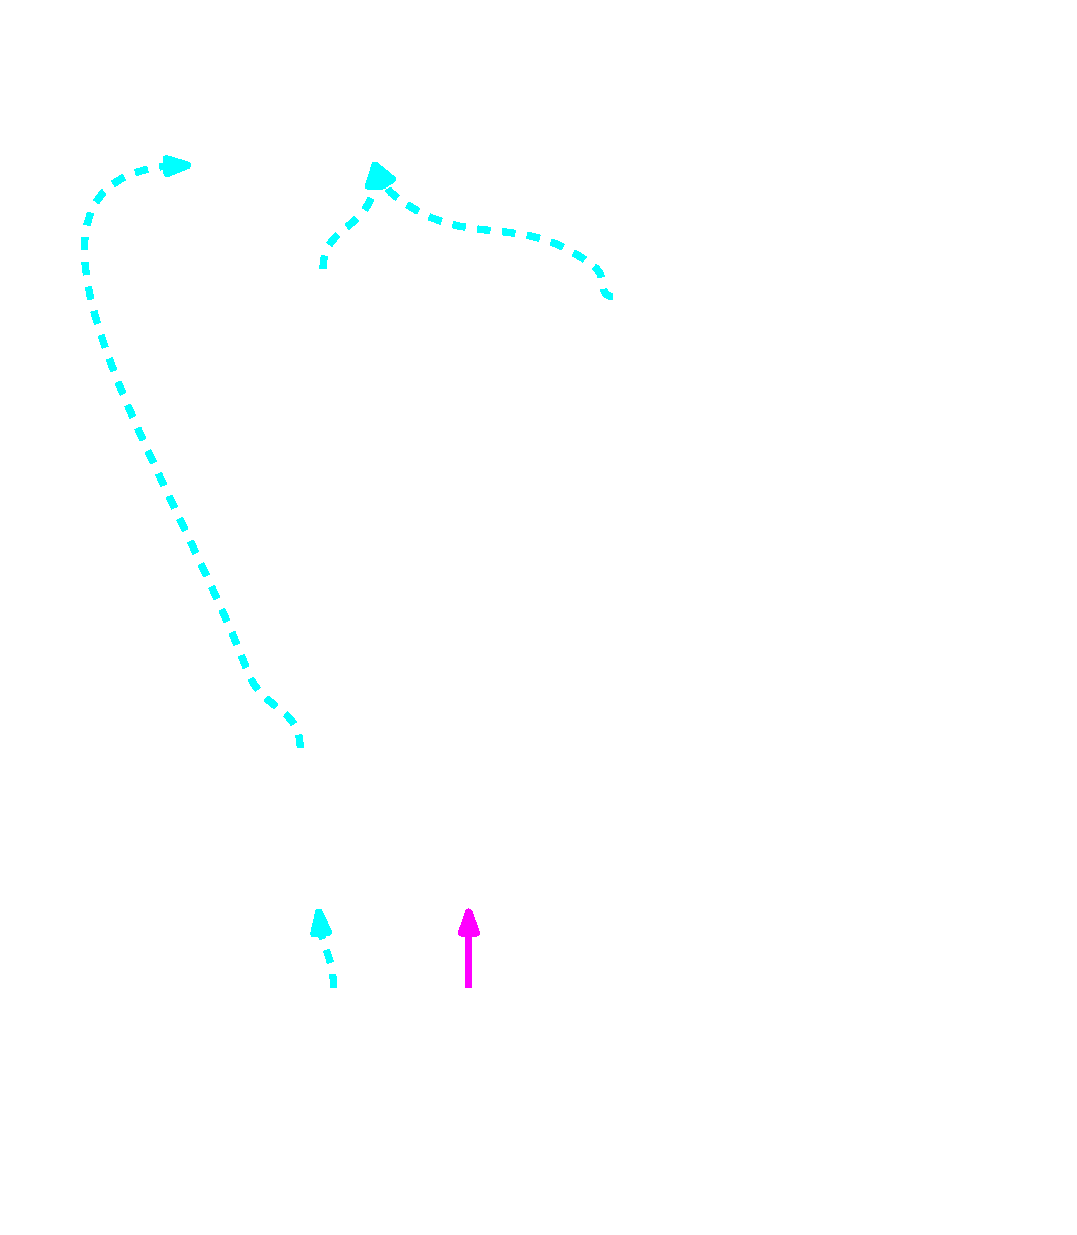
\includegraphics[width = 1.00\textwidth]{examples/ex1b/ex1b-post-isel.pdf}
    \end{figure}
\end{minipage}

\pipelinemap{IR → SelectionDAG → \codeempha{MachineDAG} → MachineInstr → MCInst}{3ex}

\end{frame}

%%%%%%%%%%%%%%%%%%%%%%%%%%%%%%%%%%%%%%%%%%%%%%%%%%%%%%%%%%%%%%%%%%%%%%%%%%%%%%%%

\begin{frame}{Before and after instruction selection}

\begin{minipage}[t]{0.50\linewidth}
    Before:
    \begin{figure}
        \vspace{-3.0ex}
        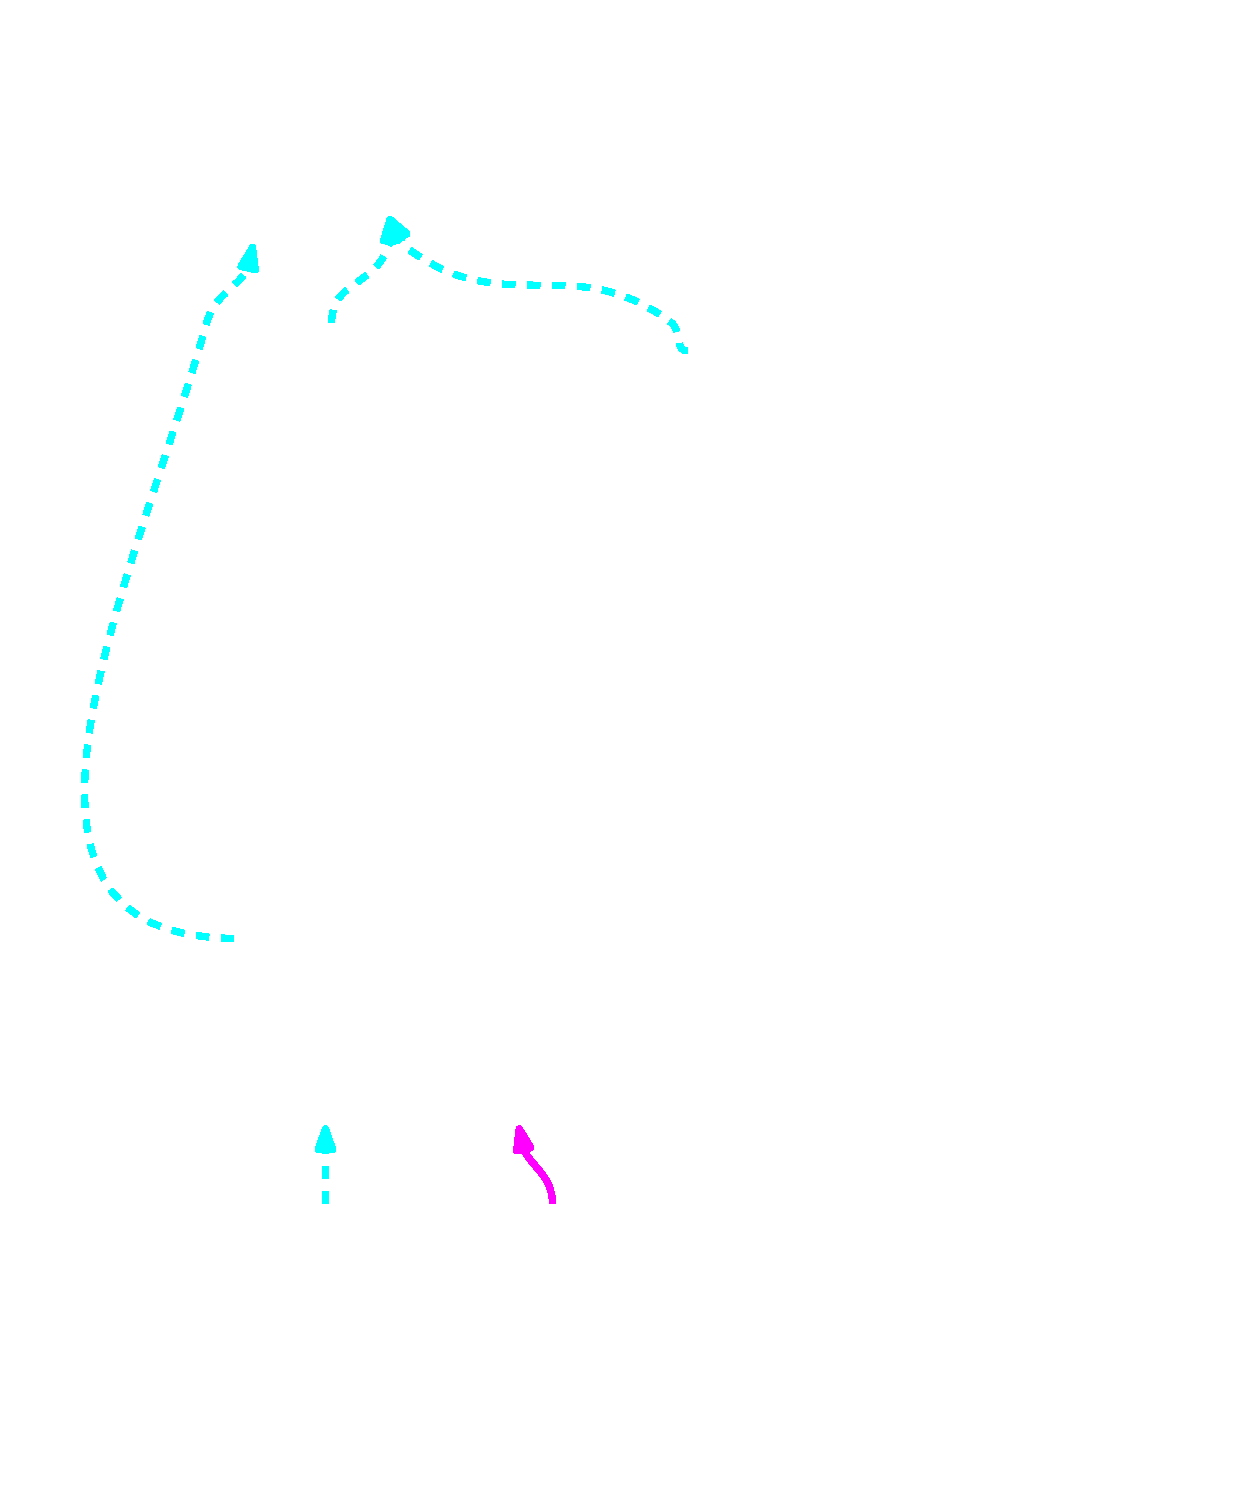
\includegraphics[width = 1.00\textwidth]{examples/ex1b/ex1b-pre-isel.pdf}
    \end{figure}
\end{minipage}
\begin{minipage}[t]{0.49\linewidth}
    After:
    \begin{figure}
        \vspace{-3.0ex}
        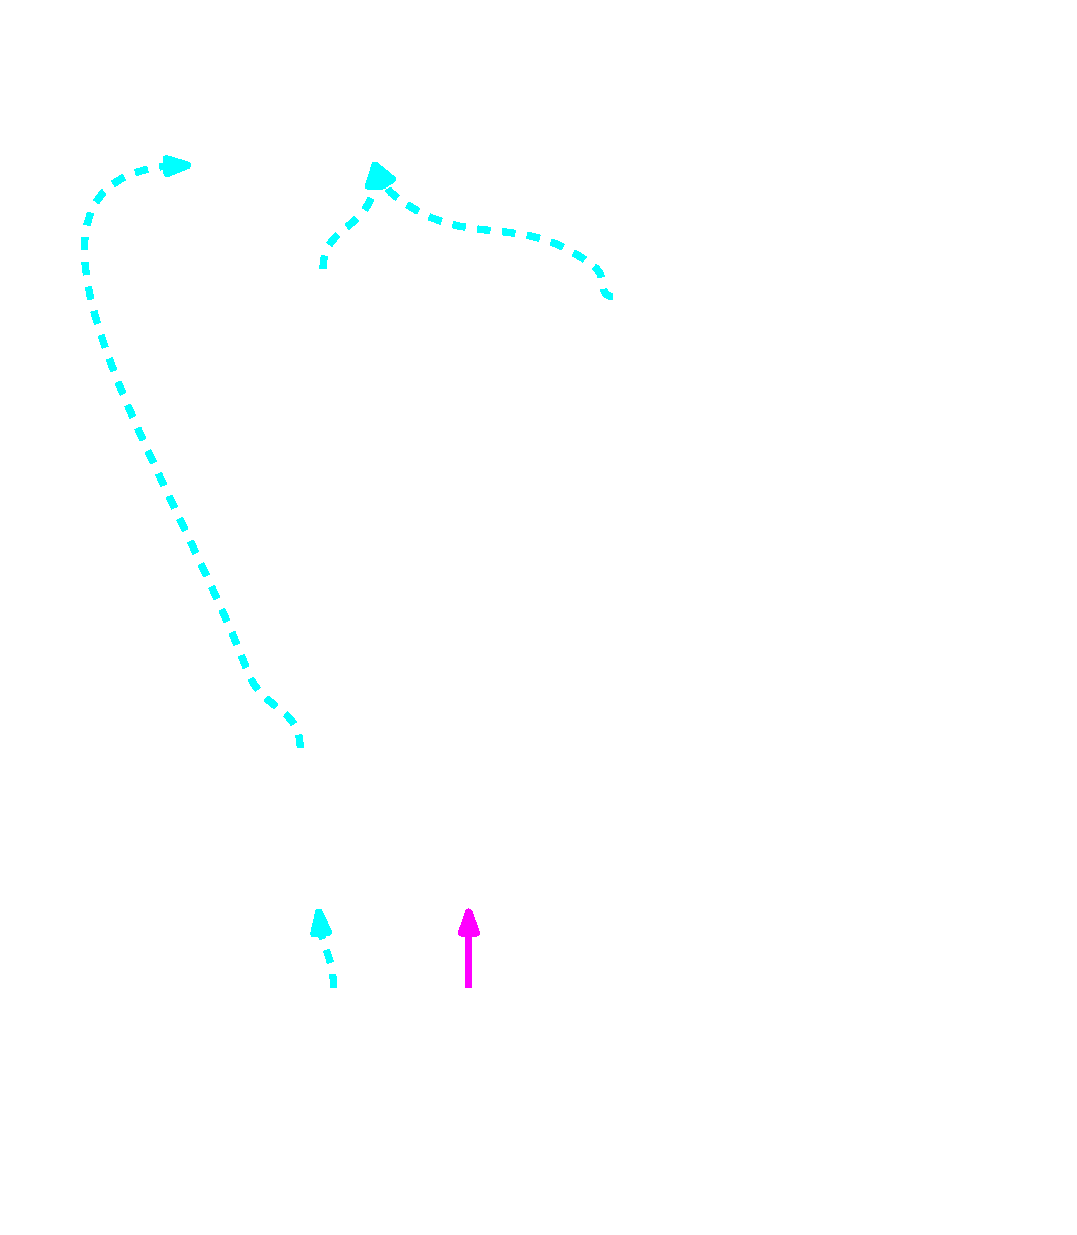
\includegraphics[width = 1.00\textwidth]{examples/ex1b/ex1b-post-isel.pdf}
    \end{figure}
\end{minipage}

\pipelinemap{IR → \codeempha{SelectionDAG} → \codeempha{MachineDAG} → MachineInstr → MCInst}{1.7ex}

\end{frame}

%%%%%%%%%%%%%%%%%%%%%%%%%%%%%%%%%%%%%%%%%%%%%%%%%%%%%%%%%%%%%%%%%%%%%%%%%%%%%%%%

\begin{frame}{A look at a MachineInstr block}

\begin{itemize}
    \item Untyped, uses register classes instead
    \begin{itemize}
        \item Virtual registers (before register allocation)
        \item Machine registers (after RA)
    \end{itemize}
    \item Target-specific instructions (LEG namespace)
    \begin{itemize}
        \item Few exceptions (TargetOpcode namespace)
    \end{itemize}
    \item Instruction operands have flags:
    \begin{itemize}
        \item Def for outputs, use for inputs
        \item Kill: last use of a value stored in a register
    \end{itemize}
\end{itemize}

\examplebox{ex1/ex1-mi.txt}

\pipelinemap{IR → SelectionDAG → MachineDAG → \codeempha{MachineInstr} → MCInst}{1.3ex}

\end{frame}
